% Created 2017-10-05 Thu 10:33
% Intended LaTeX compiler: pdflatex
\documentclass[11pt]{article}
\usepackage[utf8]{inputenc}
\usepackage[T1]{fontenc}
\usepackage{graphicx}
\usepackage{grffile}
\usepackage{longtable}
\usepackage{wrapfig}
\usepackage{rotating}
\usepackage[normalem]{ulem}
\usepackage{amsmath}
\usepackage{textcomp}
\usepackage{amssymb}
\usepackage{capt-of}
\usepackage{hyperref}
\usepackage{algpseudocode, wasysym}
\date{\today}
\title{}
\hypersetup{
 pdfauthor={},
 pdftitle={},
 pdfkeywords={},
 pdfsubject={},
 pdfcreator={Emacs 25.3.1 (Org mode 9.1.1)}, 
 pdflang={English}}
\begin{document}

\tableofcontents

\section{Lecture 1 \textit{<2017-09-05 Tue>}}
\label{sec:org90d5051}
\subsection{Algorithm}
\label{sec:org77209d8}
\begin{itemize}
\item Al-Khwarizmi (9th Century)
\item Algorismus (Latin)
\item Arithmos (Greek)
\begin{itemize}
\item Greek + Latin > Algorithm
\end{itemize}
\end{itemize}
A set of step by step instructions
\begin{enumerate}
\item Every step simple and precise
\item Produces an answer in finite time (not run forever)
\end{enumerate}
This course will be very rigorous, lots of proofs, but it will take 2-3 months to formally define algorithms, so we'll just have to be satisfied with thsi definition.
Formalized in 1930's by Turing and Church.
\begin{itemize}
\item Covered in COMP 330
\end{itemize}
Even though the concept of an algorithm is very simple and intuitive, it's not very obvious to prove things.
\begin{itemize}
\item Algorithms are an old concept, have been studied forever. Some examples are really old
\end{itemize}
\subsubsection{Examples of algorithms}
\label{sec:orgf1ee37f}
\begin{itemize}
\item Recipes
\item 1600 BC Babylonians (Factorization and square roots)
\item Euclid's Algorithm (200 BC)
\begin{itemize}
\item Finding greatest common divisor of 2 numbers
\end{itemize}
\end{itemize}
Field of theoretical computer science is much older than first computers.
\begin{itemize}
\item Really mature field.
\item Computers are just a device that helps us use these things.
\item Theoretical computer science is part of math and science and has been studied for milennials
\end{itemize}
\subsection{Teacher's website}
\label{sec:org67af729}
\url{http://www.cs.mcgill.ca/\~hatami/}
\begin{itemize}
\item He will be following the textbook.
\end{itemize}
\subsection{Stable matching}
\label{sec:orgfd61068}
n men: \(m_1, m_2, \ldots, m_n\)
n women: \(w_1, w_2, \ldots, w_n\)

Every man and woman has a ranking of people of other gender.
\subsubsection{Ex: \(n=4\)}
\label{sec:org68da5db}
\(m_1: w_3 > w_1 > w_2 > w_4\)

\(m_2: w_1 > w_4 > w_2 > w_3\)

\(m_3: w_1 > w_2 > w_4 > w_3\)

\(m_4: w_2 > w_3 > w_4 > w_1\)

\noindent\rule{\textwidth}{0.5pt}

\(w_1: m_4 > m_2 > m_1 > m_3\)

\(w_2: m_1 > m_2 > m_3 > m_4\)

\(w_3: m_2 > m_1 > m_3 > m_4\)

\(w_4: m_4 > m_1 > m_2 > m_3\)

\begin{enumerate}
\item A pairing
\label{sec:org90afa42}
\begin{itemize}
\item \(m_1+w_2\)
\item \(m_2+w_4\)
\item \(m_3+w_1\)
\item \(m_4+w_3\)
\end{itemize}
What is unstable about this? The last pair, \(m_4\) and \(w_3\).
\begin{itemize}
\item \(m_1\) and \(w_3\) prefer each other
\end{itemize}
\item Unstability:
\label{sec:org11e1e95}
If there is a pair \((m,w)\) such that
\begin{enumerate}
\item m prefers w to his current partner
\item w prefers m to her current partner
\item Selfish agents, everyone wants to be with the best possible partner they can find
\end{enumerate}
\item Problem:
\label{sec:org8866025}
Can we find a stable matching?
\end{enumerate}
\subsection{Stable Matching Algorithm}
\label{sec:org7f382d0}
while \(\exists\) a free man \uline{\(m\)}
\begin{itemize}
\item \(m\) proposes to the highest-ranked woman \uline{\(w\)} that he has not prosed yet
\item If \uline{\(w\)} is free \uline{or} prefers \(m\) to her current partner, she gets engaged to \uline{\(m\)} and her current partner becomes free
\end{itemize}
else
\begin{itemize}
\item She rejects \uline{\(m\)} and \uline{\(m\)} remains free
\end{itemize}
End while

\subsubsection{For our example:}
\label{sec:orga73f2ec}
\begin{itemize}
\item \(m_1\) proposes to \(w_3\), accepts > \(m_1+w_3\)
\item \(m_2\) proposes to \(w_1\), accepts > \(m_2+w_1\)
\item \(m_3\) proposes to \(w_1\), rejects
\begin{itemize}
\item \(m_3\) proposes to \(w_2\), accepts > \(m_3+w_2\)
\end{itemize}
\item \(m_4\) proposes to \(w_2\), rejects
\begin{itemize}
\item \(m_4\) proposes to \(w_3\), rejects
\item \(m_4\) proposes to \(w_4\), accepts > \(m_4+w_4\)
\end{itemize}
\end{itemize}
Simple example, no one broke up.
Let's change the example a bit.
\subsubsection{Modified example}
\label{sec:orgf7532a0}
\(m_1: w_3 > w_1 > w_2 > w_4\)

\(m_2: w_1 > w_4 > w_2 > w_3\)

\(m_3: w_1 > w_2 > w_4 > w_3\)

\(m_4: w_2 > w_3 > w_4 > w_1\)

\noindent\rule{\textwidth}{0.5pt}

\(w_1: m_4 > m_2 > m_1 > m_3\)

\(w_2: m_1 > m_2 > m_3 > m_4\)

\(w_3: m_2 > m_4 > m_3 > m_1\)

\(w_4: m_4 > m_1 > m_2 > m_3\)

\begin{itemize}
\item \(m_1\) proposes to \(w_3\), accepts
\item \(m_2\) proposes to \(w_1\), accepts
\item \(m_3\) proposes to \(w_1\), rejects
\begin{itemize}
\item \(m_3\) proposes to \(w_2\), accepts
\end{itemize}
\item \(m_4\) proposes to \(w_2\), rejects
\begin{itemize}
\item \(m_4\) proposes to \(w_3\), accepts, breaks up with \(m_1\)
\end{itemize}
\item \(m_1\) proposes to \(w_1\), rejects
\begin{itemize}
\item \(m_1\) proposes to \(w_2\), accepts, breaks up with \(m_3\)
\end{itemize}
\item \(m_3\) proposes to \(w_4\), accepts
\end{itemize}

\subsubsection{Why isn't this infinite?}
\label{sec:orgdc6df06}
\(P(t)\): Number of pairs \((m,w)\) such that \(m\) has not proposed to \(w\) yet at time \(t\) (number of iterations of while loop).
\(P(0)=n^2\)
\(P(1)=n^2-1\)
Is it possible that a man proposes to a woman more than once? No.
\begin{enumerate}
\item Fact:
\label{sec:org18c2c4b}
No man proposes to the same woman more than once.

Some of these proposals may never happen.

The quantity \(P\) will never go negative.
\item Fact:
\label{sec:orga29f9b3}
\(P(t)\) decreases by \(1\) at every iteration.
\item Lemma:
\label{sec:orgac9a567}
The algorithm terminates after at most \(n^2\) iterations. There will be no free men at the end.

\item Fact:
\label{sec:orgd84e48c}
Once a woman gets a proposal, she is never free again.

\(\implies\) If a man \uline{\(m\)} remains free by the end of the alg it means that at the end all women are engaged.
\(\implies\) Since there are \(n\) men and \(n\) women this means that all men are engaged as well.

\(\implies\) At the end every person is engaged.
\begin{itemize}
\item This algorithm gives us a pairing.
\begin{itemize}
\item But we need to show that this is a good pairing, that it's stable.
\end{itemize}
\end{itemize}
\end{enumerate}
\section{Lecture 2 \textit{<2017-09-07 Thu>}}
\label{sec:orgc0e9a16}
\subsection{Announcements}
\label{sec:org1b4d2ce}
\begin{itemize}
\item Lectures will be recorded.
\item Assignment 1 to come out soon, probably early next week.
\end{itemize}
\subsection{Recall:}
\label{sec:org7fec8b5}
Stable matching \(n\) men \(n\) women.
\begin{itemize}
\item Not a fundamental problem, but contains many of the elements we'll see later in this course
\end{itemize}
\subsubsection{Ex: \(n=4\)}
\label{sec:org80741a0}
\begin{center}
\begin{tabular}{lllll}
Man & Preference 1 & 2 & 3 & 4\\
\hline
\(m_1\): & \(w_3>\) & \(w_1>\) & \(w_2>\) & \(w_4\)\\
\(m_2\): & \(w_1>\) & \(w_4>\) & \(w_2>\) & \(w_3\)\\
\(m_3\): & \(w_1>\) & \(w_2>\) & \(w_4>\) & \(w_3\)\\
\(m_4\): & \(w_2>\) & \(w_3>\) & \(w_4>\) & \(w_1\)\\
\end{tabular}
\end{center}

\begin{center}
\begin{tabular}{lllll}
Woman & Pref 1 & 2 & 3 & 4\\
\hline
\(w_1\): & \(m_4>\) & \(m_2>\) & \(m_1>\) & \(m_3\)\\
\(w_2\): & \(m_1>\) & \(m_2>\) & \(m_3>\) & \(m_4\)\\
\(w_3\): & \(m_2>\) & \(m_4>\) & \(m_3>\) & \(m_1\)\\
\(w_4\): & \(m_4>\) & \(m_1>\) & \(m_2>\) & \(m_3\)\\
\end{tabular}
\end{center}

Same example as last lecture, see matching/use of algorithm in lecture 1.
Matching becomes: 

\begin{center}
\begin{tabular}{llll}
\(m_1\) & \(m_2\) & \(m_3\) & \(m_4\)\\
\hline
\(w_2\) & \(w_1\) & \(w_4\) & \(w_3\)\\
\end{tabular}
\end{center}

Top matched with bottom. Does \(w_1\) have a tendancy to break up and go with \(m_3\)? No.

\subsubsection{Last lecture we proved:}
\label{sec:org17e86bb}
\begin{enumerate}
\item The algorithm always terminates.
\begin{itemize}
\item Easy to see from the list of preferences, because we go down the list of the men's preferences, they always go down their list and never go back
\end{itemize}
\item When the algorithm terminates everybody has a partner.
\begin{itemize}
\item Won't end up with a situation where a man proposes to everyone and gets rejected
\item Women will never be free once they are initially proposed to
\item A man can't be free at the end, because that means all women we're proposed to and all women are married
\begin{itemize}
\item But same amount of women and men
\end{itemize}
\end{itemize}
\end{enumerate}

\noindent\rule{\textwidth}{0.5pt}
\subsection{Stable Matching Algorithm}
\label{sec:org5b710ef}
\subsubsection{Does this algorithm produce a stable marriage?}
\label{sec:org71c5258}
It remains to show that the output is stable.
\begin{enumerate}
\item Observation 1
\label{sec:org8fc45c7}
\begin{itemize}
\item Throughout the algorithm every man's partner gets worse and worse
\end{itemize}
\item Observation 2
\label{sec:orgbd42f22}
\begin{itemize}
\item However, for women it is the opposite
\item They accept the first proposal
\item But every partner gets better and better
\end{itemize}
\item Theorem:
\label{sec:org8ef0ebd}
The final matching is stable.
\begin{enumerate}
\item Proof:
\label{sec:orgef8f914}
Suppose not! Then there exists engaged pairs as in the following:
\begin{center}
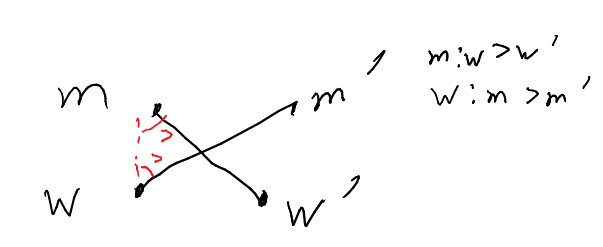
\includegraphics[width=.9\linewidth]{./Images/i1.png}
\end{center} 
But in this case \(m\) would have proposed to \(w\) before proposing to \(w'\), and as a result we know that \(w\) would not have ended up with someone worse than \(m\).
\end{enumerate}
\end{enumerate}

\subsubsection{Is this algorithm better for men or women?}
\label{sec:org80d6f65}
Let's say \((m,w)\) is valid if there exists \uline{some} stable matching that pairs \(m\) and \(w\).

\begin{enumerate}
\item Fact:
\label{sec:org7dd8440}
This algorithm matches every man with their most preferred valid \(w\) and every woman with their least preferred valid \(m\).
\begin{itemize}
\item For men, they start ambituously and go for their most preferred partner and go down the list if needed
\item For women, they start at whatever is first given and only improve if needed
\item Formal proof in textbook, won't do it in class as to spend less time on this problem
\end{itemize}
\end{enumerate}

\subsection{Notes on problems}
\label{sec:org8f2afe8}
\begin{itemize}
\item Formulate the problem as a precise mathematical problem.
\begin{itemize}
\item What is the input?
\item What is the goal?
\item Conditions we want to satisfy?
\item Everything must be precise or else we won't be able to satisfy all these things.
\end{itemize}
\item Design an algorithm
\item Analyze the algorithm:
\begin{itemize}
\item It always terminates
\begin{itemize}
\item Show that, no matter the input, it will always stop, no infinite loop
\end{itemize}
\item It outputs the correct output!
\begin{itemize}
\item In stable marriage, we showed that it is always stable
\end{itemize}
\item Running time
\begin{itemize}
\item How long does it take to terminate?
\begin{itemize}
\item For stable marriage, we could brute force and try all possible combinations and see if they're stable or not, but that would be \(n!\)
\end{itemize}
\end{itemize}
\end{itemize}
\end{itemize}

Professor won't do much on first point, about formulating problem as math. Textbook often presents the problem in a bunch of sentences for some real life thing and we need to extract the mathematical problem from there, which the professor isn't a big fan of.

\subsection{Some example problems}
\label{sec:orgb7cb980}
\subsubsection{Interval scheduling}
\label{sec:org6ff7f93}
\begin{itemize}
\item Let's say you have a room and want to rent it out
\item Bunch of offers that say the person wants to use the room from a start time to an end time
\item Want to accomodate as many people as possible, but we can't have overlap
\begin{itemize}
\item Maximize number of offers without overlap
\end{itemize}
\end{itemize}

\begin{enumerate}
\item Input:
\label{sec:org3df2719}
\begin{itemize}
\item \(n\) requests
\item Starting time \(s_1, s_2, \ldots , s_n\)
\item Finishing time \(f_1, f_2, \ldots, f_n\)
\item \uline{Such that} \(s_i<f_i\)
\end{itemize}

\item Problem
\label{sec:orge819c80}
We want to pick the max number of these tasks s.t. no two overlap. (Maximum bookings, not maximum time, not charging per hour)
\begin{center}
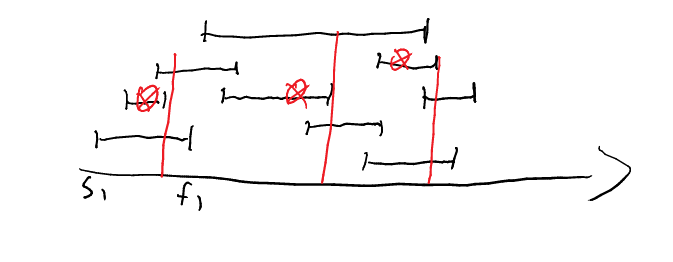
\includegraphics[width=.9\linewidth]{./Images/i2.png}
\end{center}
\begin{enumerate}
\item Algorithm?
\label{sec:org174429d}
\begin{itemize}
\item What algorithm is good for this?
\item Pick next available room that finishes the earliest and keep going
\item \textbf{Greedy algorithm}
\end{itemize}
\end{enumerate}
\end{enumerate}
\subsubsection{Weighted Interval Scheduling}
\label{sec:orgc88b1ac}
\begin{itemize}
\item Now every offer comes with some value.
\item \(v_1,\ldots,v_n\)
\begin{itemize}
\item where \(v_i\) is the value we get from accomodating the \(i^{th}\) offer.
\end{itemize}
\item \(s_1,\ldots,s_n\)
\item \(f_1,\ldots,f_n\)
\end{itemize}
Want higher value, rather than most matchings
Why is this harder to solve than the previous problem? Because the previous one is a special case of the first.
\begin{itemize}
\item Reduction = reducing this problem to the previous to get an answer
\item Setting \(v_1=\ldots=v_n=1\) solves the previous problem.
\end{itemize}
We will solve this using \textbf{Dynamic Programming}
\begin{itemize}
\item Create huge table, keep filling it up as you process input
\begin{itemize}
\item Solve solution for smaller version of problem and keep expanding based on that
\end{itemize}
\item Let's say \(A[t]=\) max value if we stop at time \(t\).
\end{itemize}
\begin{enumerate}
\item Independent set problem
\label{sec:orgc8f3d53}
\begin{center}
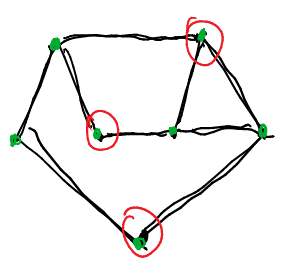
\includegraphics[width=.9\linewidth]{./Images/i3.png}
\end{center}
Independent set: A set of notes, no two are adjacent.
Find the largest independent set.
\begin{itemize}
\item Obvious way of doing it without concerning ourselves with time?
\begin{itemize}
\item Brute force
\end{itemize}
\item Without that? You can do some heuristics, but,
\begin{itemize}
\item It is widely believed that every algorithm for this problem is of brute force nature: It is more or less checking all the possible subsets?
\end{itemize}
\end{itemize}
\begin{enumerate}
\item P vs NP?
\label{sec:org492dced}
\begin{itemize}
\item Most important problem in computer science
\item Common belief: \(P\neq NP\)
\item This is an example of a problem which is believed to be NP
\end{itemize}

So that is essentially a small instruction about the types of problems we'll be seeing in this course. Next lecture we'll be formally going through running time.
\end{enumerate}
\end{enumerate}
\section{Lecture 3 \textit{<2017-09-12 Tue>}}
\label{sec:org3366c46}
\subsection{Running Time Analysis}
\label{sec:orgbad5f6f}
\begin{itemize}
\item We will be talking about running time of an algorithm.
\end{itemize}
\subsubsection{Questions}
\label{sec:org72ef659}
Thinking back without knowledge of running time, what questions can we pose?

\begin{itemize}
\item How should we measure the running time of an algorithm?
\item How can we compare the efficiency of two algorithms?
\item What should we call an \uline{efficient} algorithm?
\begin{itemize}
\item Brute force isn't efficient for finding a matching.
\item Was our algorithm for stable matchings efficient?
\item We want to understand the concept of efficiency for an algorithm.
\end{itemize}
\end{itemize}
\begin{enumerate}
\item One option:
\label{sec:orgd6f1f75}
\begin{itemize}
\item Call an algorithm efficient if it performs "fast" on \uline{"real world"} inputs.
\begin{itemize}
\item What is a real world input?
\begin{itemize}
\item Without a good/rigorous definition, then this isn't a good option.
\item Not precise, so this option doesn't work.
\end{itemize}
\end{itemize}
\end{itemize}
\item Option II:
\label{sec:orgceafac8}
\begin{itemize}
\item Take the set of all inputs of a certain size and take the average \uline{running time} of our algorithm on them.
\begin{itemize}
\item Maybe the inputs we care about are quite sparse in the set of all inputs.
\item Random inputs might be quite trivial
\begin{itemize}
\item May lead us to think we defined a good algorithm
\item But in reality what we care about is harder
\end{itemize}
\end{itemize}
\end{itemize}
\item Example: Algorithm for prime numbers
\label{sec:org2c56da4}
\begin{itemize}
\item Input: integer \(n\)
\item Output: Is \(n\) a prime number?
\begin{itemize}
\item Alg 1:
\begin{algorithmic}
	\For{$i=2$ to $n-1$}
		   \If{$n \pmod{i}=0$} return False
		   \EndIf
	\EndFor
	\State return true
\end{algorithmic}
\item Look at all the numbers between \(1,\ldots, N\)
\item How many are divisible by \({2,3,4,5,6,7}\)? \(1-\frac{1}{2}\times \frac{1}{3}\times \frac{1}{5} \times \frac{1}{7}>99\%\)
\item On average performs well
\item Worst case (prime numbers) does not perform well.
\item While this notion of average time complexity is useful, because the majority of inputs dominate the worst case ones, it is not a very good definition.
\end{itemize}
\item Better to just care about the worst case
\end{itemize}
\item Worst case time analysis
\label{sec:org521aafd}
We measure the \uline{running time} against the worst input of a given \uline{size}
\begin{itemize}
\item Want to be inddependent of implementation:
\begin{itemize}
\item We will count the number of "simple steps" (e.g. \uline{If "\(a>b\)"}, \(a:=b \times c\))
\end{itemize}
\end{itemize}
\end{enumerate}
\subsubsection{Efficiency}
\label{sec:org7680b43}
\begin{enumerate}
\item \underline{Def:}
\label{sec:org679a321}
We call an algorithm \textbf{efficient} if its running time is bounded by a polynomial \(P(n)\) for every input of \uline{size} (in number of bits) \(n\)
\begin{itemize}
\item \(n\) efficient
\item \(n^2\) good
\item \(n \log n\) good
\item \(2^n\) bad
\item \(n \log n < n^2\)
\end{itemize}
Remember that you need \(\log{n}\) bits to store a number \(n\).
\begin{itemize}
\item Objection: \uline{\(n^{100}\)} is considered efficient while it is not practical!
\item Answer: Usually the exponents are better. (Rarely see \(n^{100}\) if ever)
\end{itemize}

\noindent\rule{\textwidth}{0.5pt}
\begin{itemize}
\item Scales well
\begin{itemize}
\item Many interesting algorithms have polynomial time algorithms
\end{itemize}
\end{itemize}
\item \underline{Alternative Def:}
\label{sec:org3524c19}
Efficient is running time \(<n^3\) seems a better def as it overrules cases like \(n^{100}\)
\begin{itemize}
\item Let's say you're combining 2 algorithms, say you're running a \(n^2\) algorithm in a \(n^2\) for-loop
\begin{itemize}
\item Suddenly you're stuck with an \(n^4\) algorithm
\item This doesn't allow us to easily stick algorithms in for-loops and the like
\end{itemize}
\item This is not very robust.
\begin{itemize}
\item The choice of data structure, pseudo-code, \ldots can change the running time a bit and so this definition is not \uline{"robust"}. Result depends on implementation.
\end{itemize}
\end{itemize}
\item Example:
\label{sec:orgdbfba4f}
Input: An array \(A[0\ldots n-1]\)

Goal: Are all elements in \(A[]\) distinct?
\begin{algorithmic}
\For{$i=0$ to $n-2$}
	   \For{$j=i+1$ to $n-1$}
	   	\If{$A[i]==A[j]$}
			\State return "False"
		\EndIf
	   \EndFor
\EndFor
\State Return "True"
\end{algorithmic}
\begin{center}
\begin{tabular}{ll}
Step & Iterations\\
\hline
\(c_1\): setting \(i\) & \(n-1\)\\
\(c_2\): setting \(j\) & \(\sum_{i=0}^{n-2}\sum_{j=i+1}^{n-1}1=\frac{n(n-1)}{2}\)\\
\(c_3\): comparing \(A[i]==A[j]\) & \(\frac{n(n-1)}{2}\)\\
\(c_4\): return False & \(1\)\\
\(c_5\): return True & \(1\)\\
\end{tabular}
\end{center}

Running time: 
\begin{align*}
& n-1+\frac{n(n-1)}{2}+\frac{n(n-1)}{2}+1+1 = n^2+1
\end{align*}
\uline{Efficient}

This much accuracy is \uline{meaningless}: Each one of these commands consist of some more primitive commands and that can depend on your compiler, \ldots
\begin{itemize}
\item What matters is that this is quadratic.
\end{itemize}
\end{enumerate}

\subsubsection{Big-O notation}
\label{sec:org38f28e9}
Informally \(O(g(n))\) is the set of all functions with smaller or same order of growth.
\begin{itemize}
\item You should think of it as a set, not a value.
\item \(n \in O(n^2)\)
\item \(100n+5 \in O(n^2)\)
\item \(\frac{1}{2}n(n-1)\in O(n^2)\)
\item \(n^3 \notin O(n^2)\)
\end{itemize}
\begin{enumerate}
\item Def:
\label{sec:org606fb04}
\(f(n)\in O(g(n))\) if \(\exists n_0, c > 0\) such that \(f(n)<cg(n)\)  \(\forall n>n_0\)
\begin{center}
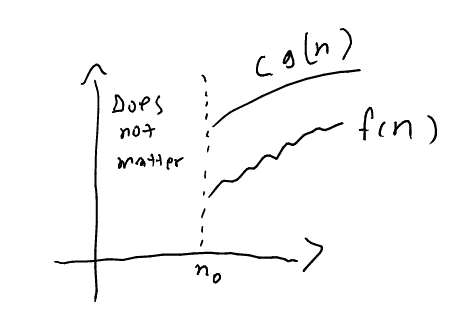
\includegraphics[width=.9\linewidth]{./Images/i4.png}
\end{center}
\item Ex:
\label{sec:orgaefb8b0}
\(100n+5 \in O(n^2)\)
\begin{enumerate}
\item Proof
\label{sec:org8bb3059}
\(100n+5 \stackrel{n\geq 5, n_0=5}{\leq} 100n+n \leq \underbrace{101}_{c=101}n\)
\end{enumerate}
\end{enumerate}

\subsubsection{\(\Omega\)-notation:}
\label{sec:orgb8f4424}
Informally \(f(n)\in \Omega(g(n))\) if \(f(n)\) grows faster or the same as \(g(n)\)
\begin{enumerate}
\item Def:
\label{sec:orga1fc485}
\(f(n) \in \Omega(g(n))\) if \(\exists n_0, c > 0\) such that \(f(n) \geq cg(n)\)  \(\forall n\geq n_0\)

(Equivalently \(g(n)\in O(f(n))\))

\begin{center}
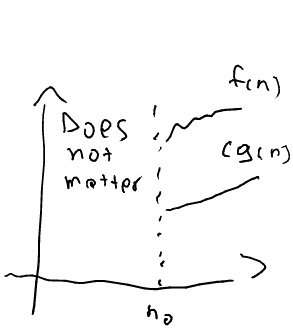
\includegraphics[width=.9\linewidth]{./Images/i5.png}
\end{center}

\item Ex:
\label{sec:orga20296b}
\(\frac{n^2}{2}-5n\in \Omega(n^2)\)
\(\frac{n^2}{2}-5n \geq \frac{1}{4} n^2 \implies c=\frac{1}{4}\)
\(\forall n \geq 20 = n_0\)
\end{enumerate}
\section{Lecture 4 \textit{<2017-09-14 Thu>}}
\label{sec:orgf9c087f}
\subsection{Recall:}
\label{sec:org522e79d}
\begin{itemize}
\item Big-Oh
\item Omega notation
\end{itemize}
\subsection{Examples}
\label{sec:org0733281}
\begin{center}
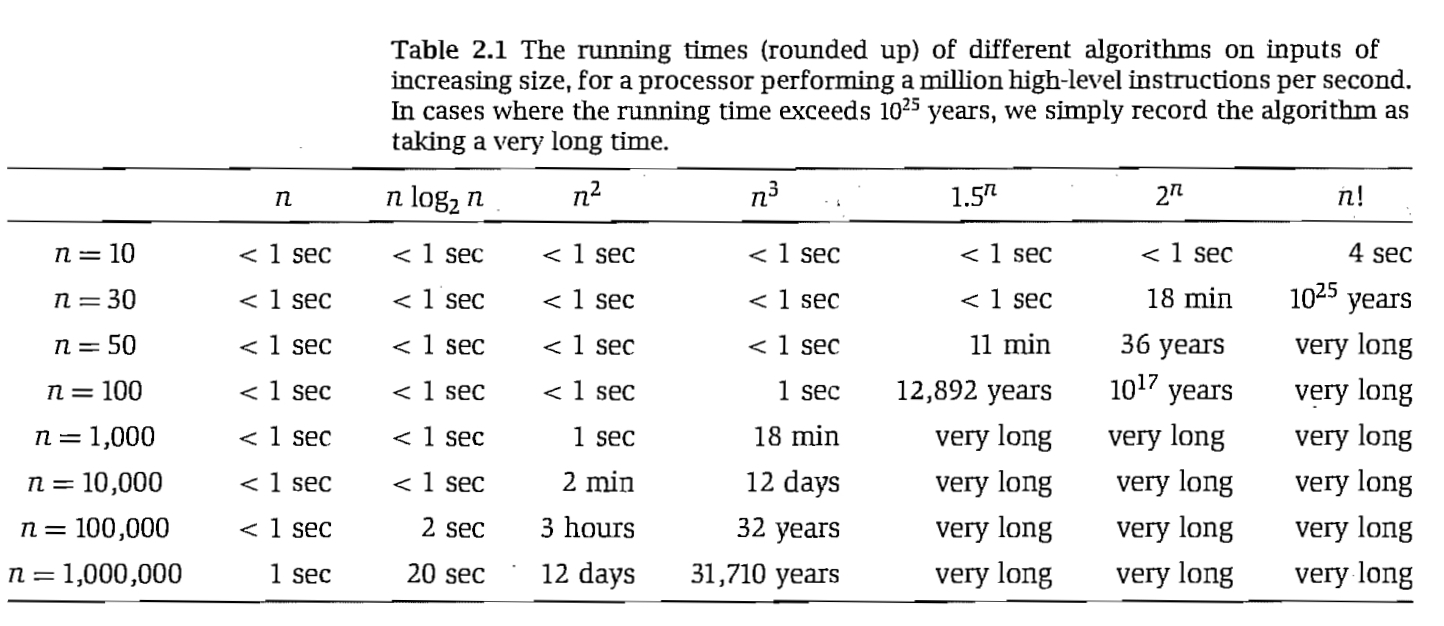
\includegraphics[width=.9\linewidth]{./Images/i6.jpg}
\end{center}
\subsection{\(\Theta\)-notation:}
\label{sec:orgc6da77f}
\(f(n)\iff f(n) = O(g(n))\) and \(f(n)=\Omega(g(n))\)
\begin{itemize}
\item Grows at the same rate as \(g(n)\)
\end{itemize}

\noindent\rule{\textwidth}{0.5pt}
Alternatively:

\(\exists n_0, c_1, c_2 \forall n>n_0\), s.t. \(c_1g(n)\leq f(n) \leq c_2 g(n)\)
\subsubsection{Examples}
\label{sec:orge3a78bd}
\begin{itemize}
\item \(2n^2+1 = \Theta(n^2)\)
\begin{enumerate}
\item \(n^2-5n+10 \leq n^2 \forall n \geq 2\)
\item \(n^2-5n+10 \geq \frac{n^2}{2} \forall n \geq 20\)
\end{enumerate}
\end{itemize}
\subsection{Theorem}
\label{sec:org8d79248}
Let \(f(n)=a_d n^d + a_{d-1}n^{d-1}+\ldots+a_1 n + a_0, a_d>0\).

Then \(f(n)=\Theta(n^d)\)
\subsubsection{Proof}
\label{sec:orge7688d4}
\begin{itemize}
\item \((f(n)=O(n^d)\)
\begin{itemize}
\item \(f(n)=a_d n^d + \ldots + a_1n + a_0 \leq \underbrace{(a_d+|a_{d-1}+\ldots+|a_0|)}_c n^d\), \(\forall n\geq 1\)
\item E.g. \(2n^2-5n+10 \leq (2+5+10)n^2\)
\end{itemize}
\item \(f(n)=\Omega(n^d)\)
\begin{itemize}
\item \(a_d n^d + a_{d-1}n^{d-1}+\ldots + a_1 n + a_0 \geq C n^d\)
\item \(c=\frac{a_d}{2}\), since \(a_d\) is controlling the growth rate of the left hand side.
\item \(\frac{a_d}{2}n^d \geq - (a_{d-1}n^{d-1}+a_{d-2}n^{d-2}+\ldots+a_0)\)
\item \(\frac{a_d}{2}n^d \geq (|a_{d-1}|+\ldots+|a_0|)n^{d-1}\), \(\forall n\geq \frac{2(|a_{d-1}+\ldots+|a_0|)}{a_d}\) (by rearranging and isolating \(n\))
\item On the other hand:
\begin{itemize}
\item \((|a_{d-1}|+\ldots+|a_0|)n^{d-1} \geq - (a_{d-1}n^{d-1}+\ldots+a_0)\)
\end{itemize}
\item Note that \(|a_r|n^{d-1} \geq -a_r n^r, r\leq d-1\)
\end{itemize}
\end{itemize}
\subsection{Little o and Little omega}
\label{sec:orgc6b3f1f}
\begin{itemize}
\item Show strict upper and lower bounds, rather than equalities
\end{itemize}
\(f(n)=o(g(n))\)
\begin{itemize}
\item \(\lim_{n\to \infty}\frac{f(n)}{g(n)}=0\)
\item Little oh implies big-Oh, but not the other way around
\end{itemize}
\(f(n)=\omega (g(n)\)
\begin{itemize}
\item \(\lim_{n\to \infty} \frac{g(n)}{f(n)} = 0\)
\end{itemize}

\noindent\rule{\textwidth}{0.5pt}
\(n^{1/100}\) vs \(\log_2 (n)^5\) 

Claim: \(\log_2(n)^5 = o(n^{1/100})\)

Proof: \(\lim_{n\to \infty}\frac{\log_2(n)^5}{n^{1/100}} = \lim_{n\to\infty}\frac{5\log(n)^4 \frac{\ln(2)}{n}}{\frac{1}{100}n^{\frac{-99}{100}}} = \ldots = 0\) (have to do L'Hopital's 4 more times)

The lesson is that anything in log grows much slower than any polynomial.
\subsection{Theorem}
\label{sec:org5908bb8}
\begin{itemize}
\item \(\forall r>1, d>0\)
\item \(n^d = o(r^n)\) (i.e. polynomials grow much slower than exponential functions)
\end{itemize}

\noindent\rule{\textwidth}{0.5pt}
\(\underbrace{n^{10000}}_{\text{Better}}\) vs \(1.0001^{n}\)
\subsection{Stable Marriage}
\label{sec:org1fb00a7}
Data structures we may use:
\begin{itemize}
\item Array \(A[0\ldots n-1]\)
\begin{itemize}
\item Operation times:
\begin{itemize}
\item Access \(A[i]: O(1)\)
\item Insert a new entry somewhere in the middle: \(O(n)\), need to shift.
\item Delete: \(O(n)\)
\item Finding an element: \(O(n)\) not sorted
\begin{itemize}
\item \(O(\log(n))\) sorted
\end{itemize}
\end{itemize}
\end{itemize}
\item Linked List
\begin{itemize}
\item Operation times:
\begin{itemize}
\item Access \(i-th\) entry: \(O(n)\)
\item Insert-delete: \(O(1)\)
\item Finding: \(O(n)\)
\end{itemize}
\end{itemize}
\end{itemize}

\begin{algorithmic}
\While {$\exists$ a free man $m$}
       \State Let $w$ be the highest-ranked woman $m$ has not proposed to yet.
       \If {$w$ is free}
       	   \State $(m,w)$ engaged
	\ElsIf{$w$ is currently engaged to $m'$}
		  \If {$w$ prefers $m$ to $m'$}
		      \State $(m',w)$ engaged
		      \State $m$ becomes free
		      \EndIf
	\EndIf	 
\EndWhile
\end{algorithmic}
\begin{itemize}
\item Input: Two (men and women) \(n\times n\) arrays (rankings)
\item Reading input \(\Theta(n^2)\) so at best we can hope \(\Theta(n^2)\) for the alg.
\item The main while loop can repeat \(O(n^2)\) times \(\implies\) To have total \(\Theta(n^2)\) time every iteration must be done in \(O(1)\).
\item How to implement?
\begin{itemize}
\item When do we know if a man is free?
\begin{itemize}
\item Can have an array of booleans of free men, but then you need for loop to check if there's a free man, which will be \(O(n)\)
\item Solution 1: Can have a linked list of free men.
\begin{itemize}
\item Delete someone from the list when they get engaged.
\item Deleting and adding is \(O(1)\) (add to front)
\end{itemize}
\item Solution 2: Using an array
\begin{itemize}
\item Have a pointer to first free man and another to last free man
\item If first man gets engaged, move pointer to the right
\item If someone becomes free, then add to end and change pointer
\item Since we never have more than \(n\) people free, can use \(\mod n\)
\end{itemize}
\end{itemize}
\end{itemize}
\end{itemize}
\section{Lecture 5 \textit{<2017-09-21 Thu>}}
\label{sec:orgbd8696b}
\subsection{Graphs}
\label{sec:org113d859}
\subsubsection{Undirected Graphs}
\label{sec:orgcd09fad}
\begin{itemize}
\item Notation \(G=(V,E)\)
\begin{itemize}
\item \(V =\) nodes (or vertices)
\item \(E =\) edges (or arcs) between pairs of nodes.
\item Captures pairwise relationship between object
\item Graph size parameters: \(n=|V|, m=|e|\)
\end{itemize}
\end{itemize}
\subsubsection{Example applications}
\label{sec:org51fdfac}
\begin{center}
\begin{tabular}{lll}
Graph & Node & Edge\\
\hline
Communication & telephone,computer & fiber optic cable\\
Circuit & gate, register, processor & wire\\
mechanical & joint & rod, beam, spring\\
financial & stock, currency & transactions\\
transportation & street intersection, airport & highway, airway route\\
internet & class C network & connection\\
game & board position & legal move\\
social relationship & person, actor & friendship, movie cast\\
neural network & neuron & synapse\\
protein network & protein & protein-protein interaction\\
molecule & atom & bond\\
\end{tabular}
\end{center}
\subsubsection{Ways of implementing in a program}
\label{sec:org5d4179d}
\begin{enumerate}
\item Adjacency matrix
\label{sec:org9a03d12}
\$n\$-by-\(n\) matrix with \(A_{uv} = 1\) if \((u,v)\) is an edge.
\begin{itemize}
\item Two representations of each edge.
\item Space proportional to \(n^2\)
\item Checking if \((u,v)\) is an edge takes \(\Theta(1)\) time
\item Identifying all edges takes \(\Theta(n^2)\) time
\item It's exactly symmetric
\end{itemize}
\item Adjacency list
\label{sec:orgd536192}
Node-indexed array of lists
\begin{itemize}
\item Two representations of each edge
\item Space is \(\Theta(m+n)\)
\item Checking if \((u,v)\) is an edge takes \(O(degree(u))\) time
\item Identifying all edges takes \(\Theta(m+n)\) time
\end{itemize}
\end{enumerate}
\subsubsection{Paths and connectivity}
\label{sec:org5dfedb1}
\begin{itemize}
\item Def. A \textbf{path} in an undirected graph \(G=(V,E)\) is a sequence of nodes \(v_1,v_2,\ldots,v_k\) with the property that each consecutive pair \(v_{i-1},v_i\) is joined by an edge in \(E\).
\item Def. A path is \textbf{simple} if all nodes are distinct.
\item Def. An undirected graph is \textbf{connected} if for every pair of nodes \(u\) and \(v\), there is a path between \(u\) and \(v\)
\end{itemize}
\subsubsection{Cycles}
\label{sec:orgcf843f6}
\begin{itemize}
\item Def. A \textbf{cycle} is a path \(v_1, v_2, \ldots, v_k\) in which \(v_1 = v_k\), \(k>2\), and the first \(k-1\) nodes are all distinct.
\end{itemize}
\subsubsection{Trees}
\label{sec:orgfb90633}
\begin{itemize}
\item Def. An undirected graph is a \textbf{tree} if it is connected and does not contain a cycle
\end{itemize}
\begin{enumerate}
\item Theorem
\label{sec:org81e10b4}
Let \(G\) be an undirected graph on \(n\) nodes. Any two of the following statements imply the third:
\begin{itemize}
\item \(G\) is connected
\item \(G\) does not contain a cycle
\item \(G\) has \(n-1\) edges
\end{itemize}
\item Rooted trees
\label{sec:org87b60dc}
\begin{itemize}
\item Given a tree \(T\), choose a root node \(r\) and orient each edge away from \(r\).
\item Importance. Models hierarchical structure
\end{itemize}
\end{enumerate}
\subsubsection{Connectivity}
\label{sec:orgbe4e405}
\begin{itemize}
\item s-t connectivity problem. Given two nodes \(s\) and \(t\), is there a path between \(s\) and \(t\)?
\item s-t shortest path problem. Given two nodes \(s\) and \(t\), what is the length of a shortest path between \(s\) and \(t\)?
\item Applications.
\begin{itemize}
\item Friendster
\item Maze traversal
\item Kevin Bacon number
\item Fewest hops in a communication network
\end{itemize}
\end{itemize}
\subsubsection{Breadth-first search}
\label{sec:orga42e2aa}
\begin{enumerate}
\item BFS intuition
\label{sec:orgd03cdb7}
Explore outward from s in all possible directions, adding nodes one "layer" at a time. At most \(n\) layers.
\item BFS algorithm
\label{sec:orgb79b549}
\begin{itemize}
\item \(L_0=\{s\}\)
\item \(L_1 =\) all neighbors of \(L_0\)
\item \(L_2 =\) all nodes that do not belong to \(L_0\) or \(L_1\), and that have an edge to a node in \(L_1\)
\item \(L_{i+1}=\) all nodes that do not belong to an earlier layer, and that have an edge to a node in \(L_i\)
\end{itemize}
\item Theorem
\label{sec:orgf66b620}
For each \(i, L_i\) consists of all nodes at distance exactly \(i\) from \(s\). There is a path from \(s\) to \(t\) iff \(t\) appears in some layer.
\item Property
\label{sec:org142026d}
Let \(T\) be a BFS tree of \(G=(V,E)\), and let \((x,y)\) be an edge of \(G\). Then, the levels of \(x\) and \(y\) differ by at most \(1\).

\item Analysis
\label{sec:org5431b85}
\begin{enumerate}
\item Theorem
\label{sec:orgba3f6eb}
The above implementation of BFS runs in \(O(m+n)\) time if the graph is given by its adjacency representation.
\item Proof
\label{sec:org5fea736}
\begin{itemize}
\item Easy to prove \(O(n^2)\) running time:
\begin{itemize}
\item At most \(n\) lists \(L[i]\)
\item Each node occurs on at most one list; for loop runs \(\leq n\) times
\item When we consider node \(u\), there are \(\leq n\) incident edges \((u,v)\), and we spend \(O(1)\) processing each edge
\end{itemize}
\item Actually runs in \(O(m+n)\) time:
\begin{itemize}
\item When we consider node \(u\), there are \(degree(u)\) incident edges \((u,v)\)
\item total time processing edges is \(\sum_{u\in V} degree(u)=2m\)
\end{itemize}
\end{itemize}
\end{enumerate}
\end{enumerate}
\section{Lecture 6 \textit{<2017-09-26 Tue>}}
\label{sec:orgcd310a5}
\subsection{Stable Marriage}
\label{sec:orgbc8f46f}
Continuation of Lecture 4: Stable Marriage algorithm analysis.
\begin{itemize}
\item Good data structure to tell if someone is free or not?
\begin{itemize}
\item Can have a linked list of all the free men, remove them when they're no longer free.
\end{itemize}
\end{itemize}
\begin{center}
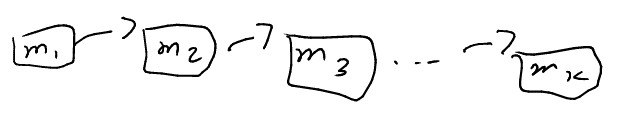
\includegraphics[width=.9\linewidth]{./Images/i7.png}
\end{center}
Initially all men are here. Finding a free man: \(O(1)\)
\begin{itemize}
\item Keep an ordered list of women sorted according to \(m\)'s preference. Keep a pointer to the first person he has not proposed to yet. (can store as a linked list, array or stack) Move pointer along to the next after proposing.
\end{itemize}
\begin{center}
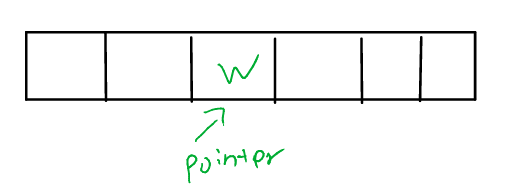
\includegraphics[width=.9\linewidth]{./Images/i8.png}
\end{center}

Now we need to know if the woman is free. Make a boolean array of women with true or false.
\begin{center}
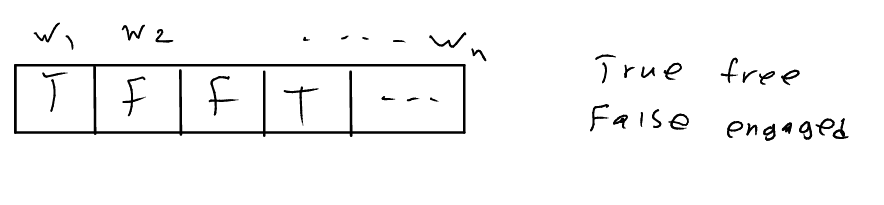
\includegraphics[width=.9\linewidth]{./Images/i9.png}
\end{center}
\begin{itemize}
\item Array telling whom \(w\) is engaged to (\(j^{th}\) entry contains who \(w_j\) is engaged to)
\end{itemize}

\begin{center}
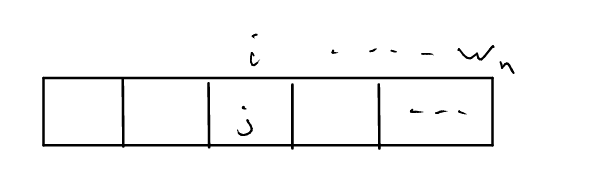
\includegraphics[width=.9\linewidth]{./Images/i10.png}
\end{center}

\begin{itemize}
\item We keep a matrix \(w[i,j] =\) the rank of \(m_j\) in the eye of \(w_i\)
\item Example: \(w_2:m_4 > m_3 > m_5>m_2 \ldots\), \(w[2,5]=3\) (don't need to do linear time)
\item If \(w_i\) prefers \(m_j\) to \(mk\) \(\iff\) \(w[i,j]<w[i,k]\)
\begin{itemize}
\item Do some "preprocessing" in the beginning to make it easier during the algorithm
\end{itemize}
\end{itemize}

With all these data structures, our algorithm can run in \(O(n^2)\)
\subsection{Priority Queue}
\label{sec:orgfb1a53d}
Say we're running a clinic and new patients come. A nurse assesses them and gives them a priority so that we know who we should see next. 

Dynamic Scenario
\begin{itemize}
\item Get elements with different priorities in an "online" matter (sometimes you get new data, not all given to you in the beginning)
\item Once in awhile we can serve the element with the highest priority (and remove from the set)
\end{itemize}

\noindent\rule{\textwidth}{0.5pt}
We have a set \(S\).
\begin{itemize}
\item Initially \(S=\emptyset\)
\item At every step either
\begin{itemize}
\item A new number is added to \(S\).
\item or the smallest number is removed from \(S\).
\end{itemize}
\end{itemize}

Some ideas:
\begin{itemize}
\item An unsorted list:
\begin{itemize}
\item Inserting a new element \(O(1)\)
\item Removing the minimum: \(O(n)\) (\(n\) elements in the list, have to find smallest)
\item Too costly, not good.
\end{itemize}
\item Sorted list:
\begin{itemize}
\item Inserting a new element \(O(n)\)
\begin{itemize}
\item With an array, need to shift all elements.
\item Linked list (no binary search)
\end{itemize}
\item Removing the smallest \(O(1)\).
\end{itemize}
\end{itemize}
\subsubsection{Heap Data Structure}
\label{sec:org4973058}
A balanced binary tree
\begin{itemize}
\item All levels are full except the last level which is filled \textbf{from left to right}
\item Every node is \(\geq\) its parent
\item Ex:
\end{itemize}
\begin{center}
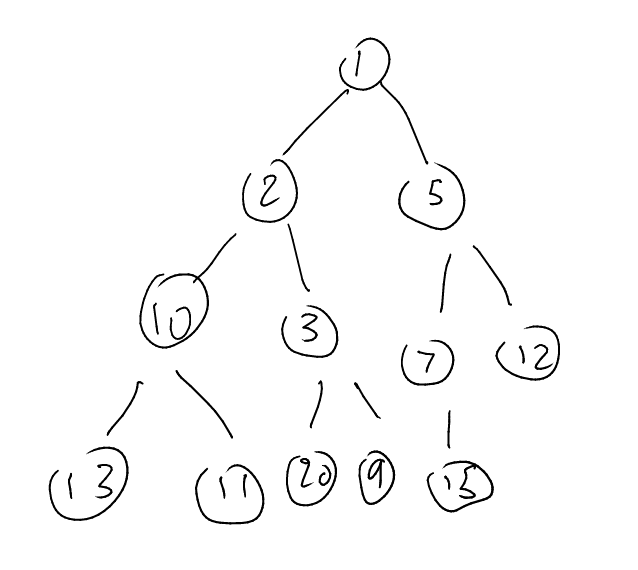
\includegraphics[width=.9\linewidth]{./Images/i11.png}
\end{center}

Can be implemented with an array. Fill left to right.

\begin{center}
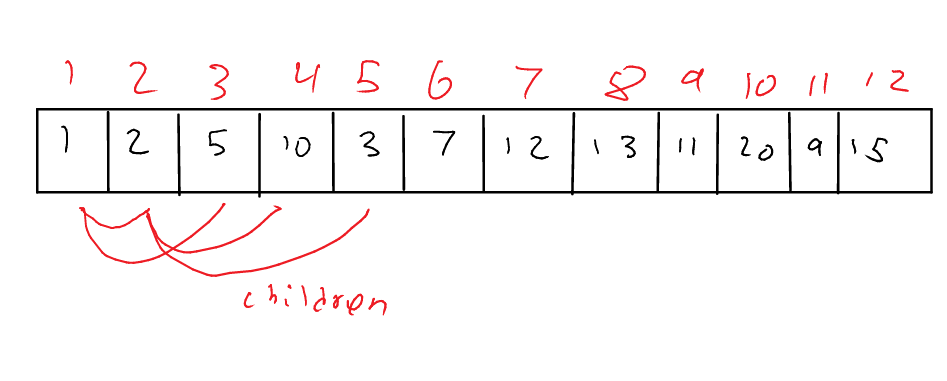
\includegraphics[width=.9\linewidth]{./Images/i12.png}
\end{center}

Where are the children of entry \(i\)? \(2i, 2i+1\) (convenient)

\noindent\rule{\textwidth}{0.5pt}
What do we do when a new number arrives? Say \uline{insert(4)}
\begin{itemize}
\item Naturally we want to put it in the next available place "\(n^{th}\)" if \(n\) is the updated \# of nodes
\end{itemize}

\begin{center}
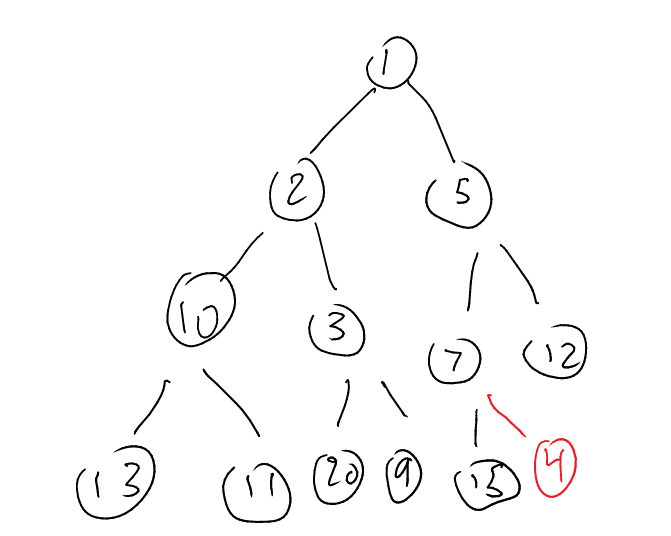
\includegraphics[width=.9\linewidth]{./Images/i13.png}
\end{center}

But 4 is smaller than its parent. How to fix? Swap with parent.

\begin{center}
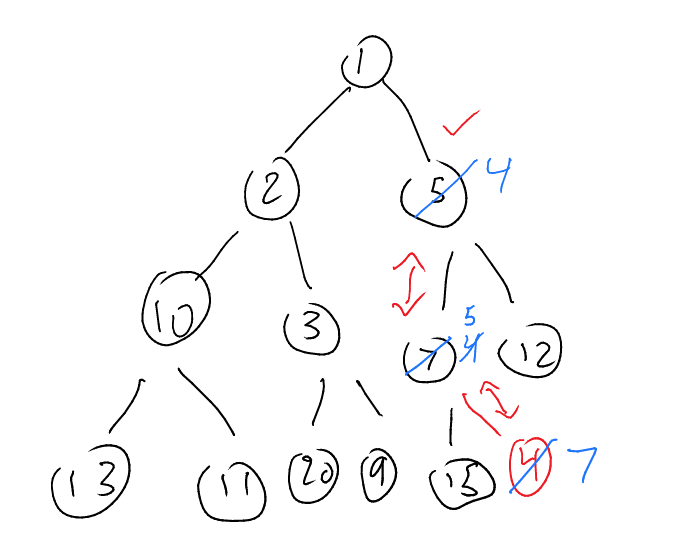
\includegraphics[width=.9\linewidth]{./Images/i14.png}
\end{center}

We will call this operation Heapify-Up.
\begin{algorithmic}
\State Heapify-Up$(H,i)$ // $i$ is index
\If {$i>1$} 
    \State let $j=parent(i)=\lfloor \frac{i}{2} \rfloor $
\If {$H[i]<H[j]$}
    \State swap$(H[i],H[j])$
    \State Heapify-Up$(H,j)$
\EndIf
\EndIf
\end{algorithmic}
Running time of Heapify-Up: \(O(\log n)=O(\text{Height of the tree})\)

\noindent\rule{\textwidth}{0.5pt}
How do we remove the minimum?
\begin{itemize}
\item Insert last element at head and then swap with smallest child until the tree is balanced
\end{itemize}
\begin{center}
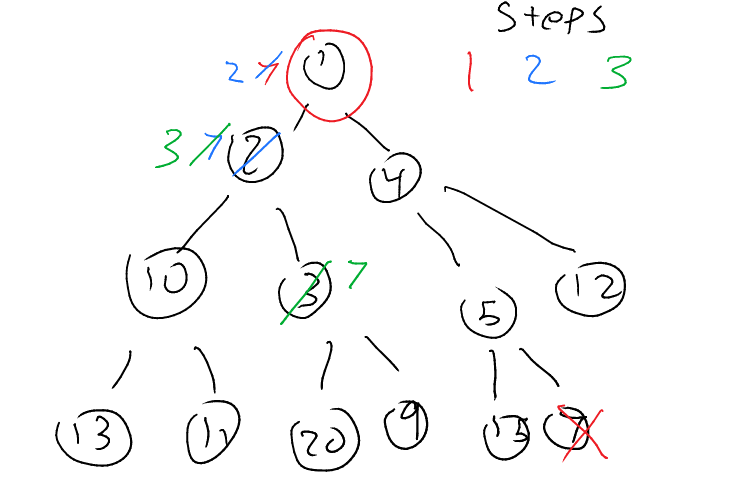
\includegraphics[width=.9\linewidth]{./Images/i15.png}
\end{center}

\begin{algorithmic}
\State Heapify-down$(H,i)$
\State $n=$ length$(H)$
\If {$2i>n$} // Elements $> n/2$ have no children
    \State Terminate
\ElsIf {$2i+1 \leq n$}
       \State $left=2i, right = 2i+1$
       \If {$H[left]<H[right]$}
       	   \State $j=left$
	   \Else 
	   \State $j=right$
	   \EndIf
\Else //$(n=2i)$
      \State $j=left=2i$
\EndIf
\If {$H[j]<H[i]$}
    \State swap$(H[j],H[i])$
    \State Heapify-down$(H,j)$
\EndIf
\end{algorithmic}

\noindent\rule{\textwidth}{0.5pt}
Q: How can we use this data structure to sort a list of \(n\) numbers?

Answer: Insert the elements one by one and then extract the minimums one by one.
\begin{itemize}
\item Running time? \(2n O(\log n)\)
\begin{itemize}
\item \(O(n\log n)\)
\end{itemize}
\end{itemize}
\section{Lecture 7 \textit{<2017-09-28 Thu>}}
\label{sec:orge4950d4}
\subsection{Graph Exploration Algorithms}
\label{sec:org76546e5}
\subsubsection{Breadth-First-Search (BFS)}
\label{sec:org5d41934}
\begin{center}
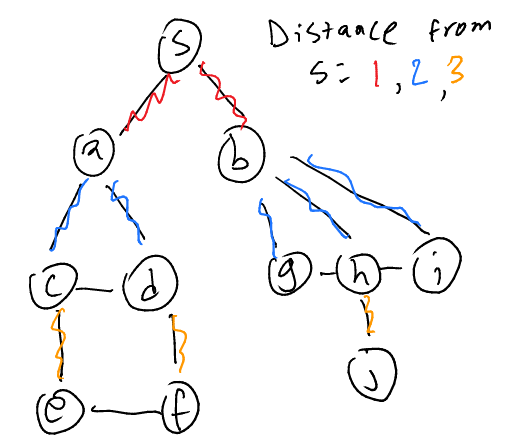
\includegraphics[width=.9\linewidth]{./Images/i16.png}
\end{center}

Also tells you length of shortest path from s to any vertex.
\begin{itemize}
\item We explore according to the distance from s.
\item How to implement this?
\end{itemize}

\noindent\rule{\textwidth}{0.5pt}
\begin{algorithmic}
  \State BFS(G)
  \For {every vertex v in G}
  \If {v is unexplored}
  \State Mark v as explorerd
  \State BFS.vertex(v)
  \State connected-comp$++$
  \EndIf
  \EndFor
\end{algorithmic}

\noindent\rule{\textwidth}{0.5pt}
\begin{algorithmic}
  \State BFS-vertex(v)
  \State Make a list of all the unexplored neighbors of v.
  \State Mark every vertex in this list as explored
  \For {every u in this list}
  \State BFS-Vertex(u)
  \EndFor
\end{algorithmic}
Recursive way above does not work?

A good way to implement this is to keep the newly discovered vertices in a queue (FIFO, first in first out).
\begin{algorithmic}
  \State BFS-Vertex(v)
  \State Add v to the queue
  \While {queue is not empty}
        \State Pick the first vertex u in the queue.
        \State Mark all unexplored neighbors of u as explored and add
        them to the queue
  \EndWhile
\end{algorithmic}
\begin{center}
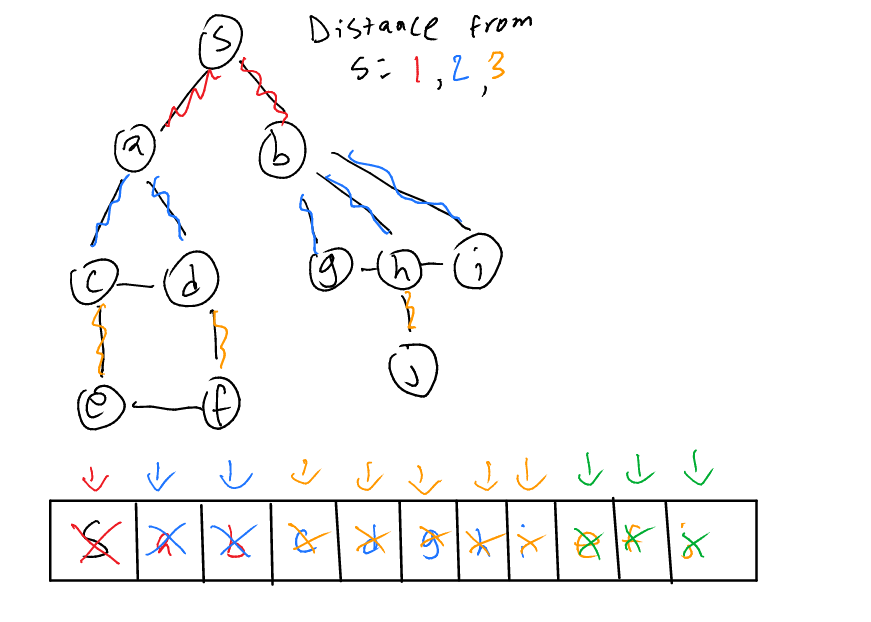
\includegraphics[width=.9\linewidth]{./Images/i17.png}
\end{center}

\subsubsection{Depth-First-Search (DFS)}
\label{sec:org5d7e15e}
We go in a path discovering new vertices until we reach a dead-end, and then we step back \(\ldots\)

\noindent\rule{\textwidth}{0.5pt}
\begin{algorithmic}
  \State DFS(u)
  \For {every edge (u,v)}
        \If{v is unexplored}
                \State{mark v as explored}
                \State{DFS(v)}
        \EndIf
  \EndFor        
\end{algorithmic}
\begin{center}
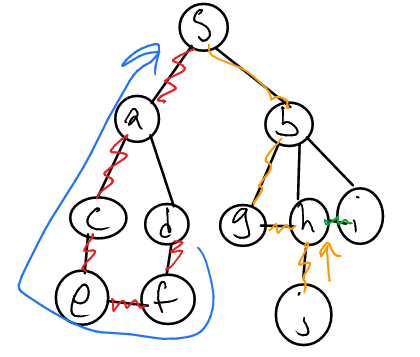
\includegraphics[width=.9\linewidth]{./Images/i18.png}
\end{center}

\noindent\rule{\textwidth}{0.5pt}
Non-recursive DFS: Every time we discover a new vertex we put it at the top of a stack (FILO, first in last out).
\subsection{Data Structure for Graphs}
\label{sec:org1406ce6}
What data structure to use for graphs?
\begin{itemize}
\item Adjacency Matrix
\begin{equation*}
  A[u,v] =
  \begin{cases}
    1 & \text{if }(u,v)\in E
    \\ 0 & \text{if }(u,v)\notin E
  \end{cases}
\end{equation*}
\begin{itemize}
\item Pros: very easy to see if u is connected to v
\item Cons: IF the graph has few edges it is wasteful. \(O(n^2)\) bits of memory.
\end{itemize}
\end{itemize}

\noindent\rule{\textwidth}{0.5pt}
\begin{itemize}
\item For every vertex v we keep a list of all edges (u,v) incident to v
\item Pros: easy to find the neighbors
\begin{itemize}
\item Doesn't take much memory if the graph is sparse
\end{itemize}
\item Cons: Takes \(O(n)\) to see if u is adjacent to v.
\end{itemize}
\subsection{Bipartites}
\label{sec:org7d6a93a}
An undirected graph is called \uline{bipartite} if we can \uline{partition} the vetices into two parts \(R\) and \(B\) such that all the edges are between \(R\) and \(B\)
\begin{center}
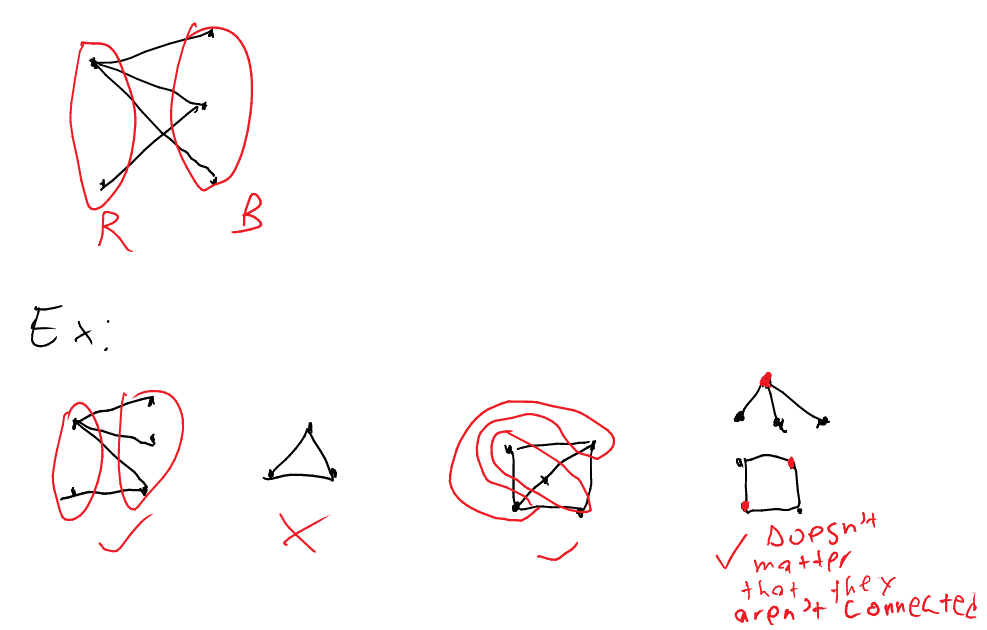
\includegraphics[width=.9\linewidth]{./Images/i19.png}
\end{center}
\subsubsection{Testing for bipartites}
\label{sec:orgad94b1c}
How can we test to see if \(G\) is bipartite? Label one vertex in \(R\) then:
\begin{itemize}
\item Look at neighbors to see if they're supposed to be \(R\) or \(B\)
\end{itemize}
\begin{center}
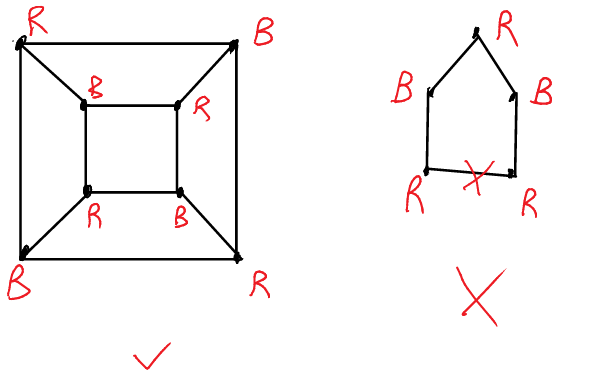
\includegraphics[width=.9\linewidth]{./Images/i20.png}
\end{center}

\noindent\rule{\textwidth}{0.5pt}
\begin{algorithmic}
  \State DFS\_Bipartitite(G)
  \For {every vertex u in G}
        \If{u is not explored}
                \State color[u] = ``R''
                \State mark u as explored
                \State DFS(u)
        \EndIf
 \EndFor
 \If{not declared ``non-bipartite'' yet}
        \State declare ``bipartite''
\EndIf
      \end{algorithmic}

\noindent\rule{\textwidth}{0.5pt}
\begin{algorithmic}
  \For{each edge (u,v)}
  \If{v is not explored}
  \State Mark v as explored
  \State color v differently from color[u]
  \State DFS(v)
  \ElsIf{color[u]=color[v]}
  \State declare ``non-bipartite''
  \EndIf
  \EndFor
\end{algorithmic}
This is called proper two coloring of a graph.
\subsection{Directed Graphs}
\label{sec:org2beb67f}
Every edge has an orientation.
\begin{center}
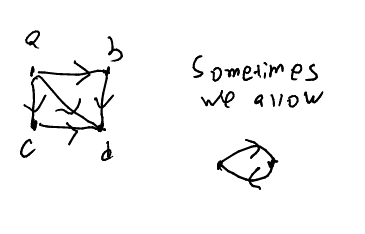
\includegraphics[width=.9\linewidth]{./Images/i21.png}
\end{center}

\subsubsection{Data Structure:}
\label{sec:org31fb246}
For every vertex keep two lists: the edge going out, the edges coming into that vertex
Given two vertices, s and t, is there a path from s to t?
\begin{itemize}
\item say s=a t=d
\item yes in the graph
\item But there is no path from d to a.
\end{itemize}
We can use the "directed" version of DFS to solve this problem: We run DFS(s) if t is explored then such a path exists otherwise it doesn't.

Def: A directed graph is called strongly connected if for every u and v there is a path from u to v. (can go from anywhere to anywhere)

\begin{center}
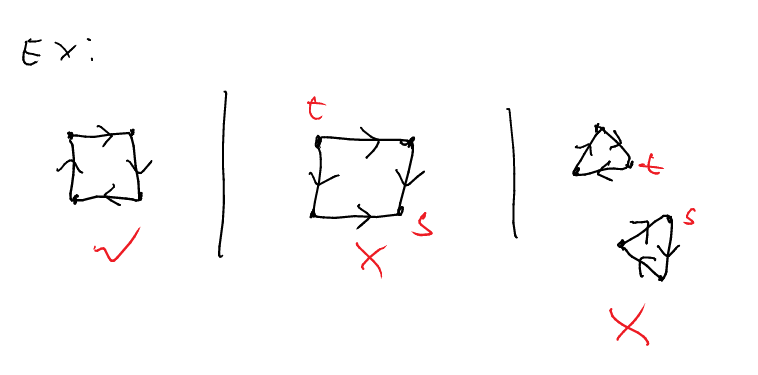
\includegraphics[width=.9\linewidth]{./Images/i22.png}
\end{center}

\noindent\rule{\textwidth}{0.5pt}
Q: Given \(G\), how can we tell if it is strongly connected?
\begin{itemize}
\item Pick a vertex s
\item Run DFS(s) in \(G\)
\item If there is any unexplored vertex then "not strongly connected"
\item Run DFS(s) in \(G^{rev}\) (same as \(G\), but with directions reversed)
\item If \(\exists\) any unexplored vertex then "not strongly connected"
\item Otherwise declare "G is strongly connected"
\end{itemize}
\section{Lecture 8 \textit{<2017-10-03 Tue>}}
\label{sec:orgce8c961}
\subsection{Directed Graphs}
\label{sec:org0c326f6}
\begin{itemize}
\item Each edge has a direction (seen last class)
\item Not symmetric, edge from u to v means no edge from v to u.
\end{itemize}
\subsubsection{Graph search}
\label{sec:org3481cd2}
\begin{itemize}
\item Directed reachability
\begin{itemize}
\item Find all nodes reachable from a given node
\end{itemize}
\item Directed s-t shortest path problem
\begin{itemize}
\item Given two nodes, what is length of shortest path between them
\end{itemize}
\item BFS extends naturally to directed graphs
\item Web crawler
\begin{itemize}
\item Start from web page s. Find all web pages linked from s
\end{itemize}
\end{itemize}
\subsubsection{Strong Connectivity}
\label{sec:org6b2c599}
\begin{itemize}
\item Node u and v are \textbf{mutually reachable} if there is a path from u to v and also a path from v to u.
\item A graph is \textbf{strongly connected} if every pair of nodes is mutually reachable.
\end{itemize}
\begin{enumerate}
\item Lemma
\label{sec:org16cbc76}
Let s be any node. G is strongly connected iff every node is reachable from s, and s is reachable from every node.
\begin{itemize}
\item Proof: \(\implies\) Follows from definition
\item \(\impliedby\) Path from u to v: concatenate u-s path with s-v path
\begin{itemize}
\item Path from v to u: concatenate v-s path with s-u path
\end{itemize}
\end{itemize}
\item Algorithm
\label{sec:org5901e3e}
\begin{enumerate}
\item Theorem
\label{sec:org19c2752}
Can determine if G is strongly connected in \(O(m+n)\) time.

Proof:
\begin{itemize}
\item Pick any node \(s\)
\item Run BFS from \(s\) in \(G\)
\item Run BFS from s in \(G^{rev}\)
\item Return true iff all nodes reached in both BFS executions
\item Correctness follows immediately from previous lemma
\item Has running time of BFS \(O(m+n)\)
\end{itemize}
\end{enumerate}
\end{enumerate}
\subsection{Directed Acyclic Graphs}
\label{sec:orgfa9c50b}
\begin{itemize}
\item A \textbf{DAG} is a directed graph that contains no directed cycles
\begin{itemize}
\item Good for modeling dependencies, like a course's prerequisites
\end{itemize}
\item Ex. Precedence constraints: edge \((v_i,v_j)\) means \(v_i\) must precede \(v_j\).
\begin{itemize}
\item Precedence constraints imply no cycle
\end{itemize}
\item A \textbf{topological order} of a directed graph \(G=(V,E)\) is an ordering of its nodes as \(v_1,v_2,\ldots,v_n\) so that for every edge \((v_i,v_j)\) we have \(i<j\)
\end{itemize}
\subsubsection{Lemma}
\label{sec:orgaac5ffa}
If \(G\) has a topological order, the \(G\) is a DAG.

Proof (by contradiction)
\begin{itemize}
\item Suppose \(G\) has a topological order \(v_1,\ldots,v_n\) and that \(G\) also has a directed cycle \(C\).
\item Let \(v_i\) be the lowest-indexed node in \(C\) and let \(v_j\) be the node just before \(v_i\): thus \((v_j,v_i)\) is an edge.
\item By our choice of \(i\), we have \(i<j\)
\item On the other hand, since \((v_j,v_i)\) is an edge and \(v_1,v_2,\ldots,v_n\) is a topological order, we must have a contradiction. \lightning
\end{itemize}
\subsubsection{Lemma}
\label{sec:org2fe98d6}
If \(G\) is a DAG, then \(G\) has a node with no incoming edges.

Proof (by contradiction)
\begin{itemize}
\item Suppose \(G\) is a DAG and every node has at least one incoming edge.
\item Pick any node \(v\), begin following edges backward from \(v\). Since \(v\) has at least one incoming edge \((u,v)\) we can walk backward to \(u\).
\item Since \(u\) has at least one incoming edge \((x,u)\) we can walk backward to \(x\)
\item Repeat until we visit a node, say \(w\), twice.
\item Let \(C\) denote the sequence of nodes encountered between successive visits to \(w\). \(C\) is a cycle. \lightning
\end{itemize}
\subsubsection{Lemma}
\label{sec:org25f8330}
If \(G\) is a DAG, then \(G\) has a topological ordering.

Proof (by induction on \(n\))
\begin{itemize}
\item Base case: true if \(n=1\)
\item Given DAG on \(n>1\) nodes, find a node \(v\) with no incoming edges
\item \(G \setminus \{v\}\) is a DAG, since deleting \(v\) cannot create cycles
\item By inductive hypothesis, \(G\setminus\{v\}\) has a topological ordering.
\item Place \(v\) first in topological ordering: then append nodes of \(G\setminus \{v\}\) in topological order. This is valid since \(v\) has no incoming edges.
\end{itemize}
\begin{enumerate}
\item Algorithm
\label{sec:orga6994ab}
To compute a topological ordering of \(G\)
\begin{itemize}
\item Find a node \(v\) with no incoming edges and order it first
\item Delete \(v\) from \(G\)
\item Recursively compute a topological ordering of \(G\setminus \{v\}\) and append this order after \(v\)
\item Running time: \(O(n)\) for each call, calling exactly \(n\) times. So algorithm runs in \(O(n^2)\). Lots of running time if the graph is sparse, not many edges. If we reimplement this more carefully, we can get \(O(m+n)\), with \(m\) being the number of edges. Note that making an algorithm run faster usually requires more space.`
\end{itemize}
\item Theorem
\label{sec:orga94578e}
Algorithm finds a topological order in \(O(m+n)\) time

Proof:
\begin{itemize}
\item Maintain the following information:
\begin{itemize}
\item \(count[w] =\) remaining number of incoming edges
\item \(S=\) set of remaining nodes with no incoming edges
\end{itemize}
\item Initialization: \(O(m+n)\) via single scan through graph.
\item Update: to delete \(v\)
\begin{itemize}
\item Remove \(v\) from \(S\)
\item Decrement \(count[w]\) for all edges from \(v\) to \(w\) and add \(w\) to \(S\) if \(count[w]\) hits \(0\)
\item This is \(O(1)\) per edge
\end{itemize}
\end{itemize}
\end{enumerate}
\section{Lecture 9 \textit{<2017-10-05 Thu>}}
\label{sec:org18f89f7}
\subsection{Greedy Algorithm}
\label{sec:org9da62ef}
\begin{itemize}
\item In every step, it tries to be myopic and optimize its current goal/step
\item Doesn't care about the future
\end{itemize}
\subsubsection{Interval scheduling}
\label{sec:org74bb4f6}
\begin{itemize}
\item Have a class room and a microscope
\item Every request has a starting time and finishing time \(\{1,\ldots, n\}\), \((s_i,f_i)\)
\item Def. \(i\) and \(j\) are \uline{compatible} \((i+j)\) when \(f_i \leq s_j\) or \(f_j \leq s_i\)
\item Subset of requests is \uline{compatible} if every point of requests are compatible.
\item Maximum sized compatible subset is the \uline{optimal subset}
\end{itemize}

\noindent\rule{\textwidth}{0.5pt}
\begin{enumerate}
\item Pick \(s(i)\) with earliest request
\begin{itemize}
\item Might not give an optimal solution if the request that begins the earliest goes until the end, not allowing any of the other requests to be fulfilled.
\begin{center}
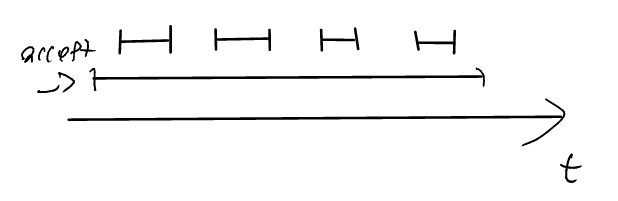
\includegraphics[width=.9\linewidth]{./Images/i23.png}
\end{center}
\end{itemize}
\item \(f(i)-s(i)\) is the smallest 
\begin{itemize}
\item Can be problematic if the smallest is in between 2
\end{itemize}
\begin{center}
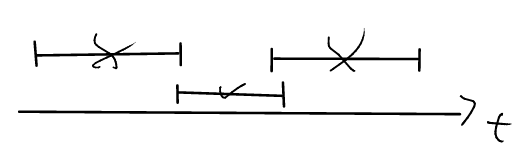
\includegraphics[width=.9\linewidth]{./Images/i24.png}
\end{center}
\item For each request compute the \# of requests it overlaps with. Pick the one with the smallest number.
\begin{itemize}
\item Still problematic
\begin{center}
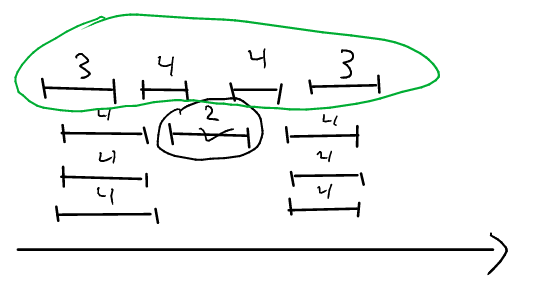
\includegraphics[width=.9\linewidth]{./Images/i25.png}
\end{center}
\end{itemize}
\item \uline{Accept} (greedy rule) requests \(i\) for which \(f(i)\) is the smallest.
\begin{itemize}
\item Sort requests so that \(f(i_1)\leq f(i_2)\leq \ldots \leq f(i_n)\)
\item This one works
\end{itemize}
\end{enumerate}
\begin{algorithmic}
  \State $A = \emptyset$
  \For {$j=1$ to $n$}
  \If {j is compatible with $A$}
  \State $A \gets A \cup \{j\}$
  \EndIf
  \EndFor
  \State return A
\end{algorithmic}

\noindent\rule{\textwidth}{0.5pt}
\subsubsection{{\bfseries\sffamily TODO} clean up this section}
\label{sec:orgb507002}
Running time of method 4:
\begin{itemize}
\item Sort : \(O(n\log n)\)
\item \(f(j)\geq f(j^*) \forall i \in A, f(i) \leq f(j^*) \gets O(n)\)
\begin{center}
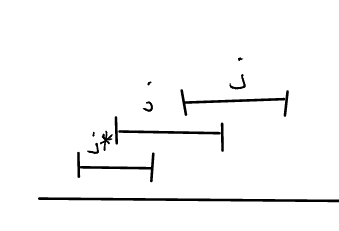
\includegraphics[width=.9\linewidth]{./Images/i26.png}
\end{center}
\end{itemize}
\subsubsection{Theorem}
\label{sec:org528e080}
This greedy algorithm returns the optimal subset.
$$\underbrace{|A|}_{\text{optimal}} = |O| - \text{optimal subset}$$
\begin{itemize}
\item "stays ahead"
\item \(|A|=k, |O|=n\), assume \(k<m\)
\item \(O\) is ordered by their starting and finishing time for every \(j \in O\), \(f(i_1 \in A) \leq f(j)\)
\end{itemize}

\begin{enumerate}
\item Lemma.
\label{sec:orgb7ab513}
For all \(r \leq k\), \(f(i_r) \leq f(j_r)\)
\begin{enumerate}
\item Proof
\label{sec:orgefd7420}
\begin{itemize}
\item \(r=1 f(\underbrace{i_1}_A) \leq f(\underbrace{j_1}_O)\) Works
\item This greedy algorithm returns the optimal subset \(r-1\) i.e. \(f(i_{r-1})\leq f(j_{r-1})\).
\item But this contradicts \(f(i_r) \geq f(j_r) \implies f(i_r)\leq (j_r)\)
\end{itemize}
\begin{center}
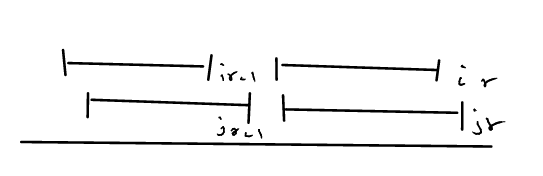
\includegraphics[width=.9\linewidth]{./Images/i27.png}
\end{center}


\begin{itemize}
\item \(A: i_1 \ldots i_k\)
\item \(O: j_1 \ldots j_k j_{k+1} \ldots\)
\item Apply the lemma with \(r=k\) so \(f(i_k)\leq f(j_k)\)
\end{itemize}
\begin{center}
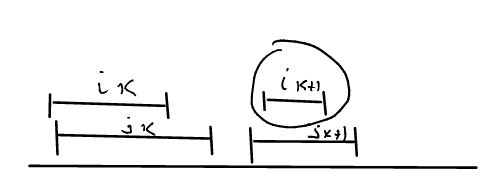
\includegraphics[width=.9\linewidth]{./Images/i28.png}
\end{center}
This contradicts \(k<m\)! Thus \(m=k\)
\begin{itemize}
\item Sort \(O\) by starting time, it's also sorted by finishing time
\end{itemize}
\end{enumerate}
\end{enumerate}
\subsubsection{Satisfying requests}
\label{sec:org9236b34}
Given requests, how many resources do we need to satisfy all of them?
\begin{itemize}
\item Def. depth is the maximum number of requests that have a common point in the time line.
\end{itemize}
\begin{enumerate}
\item Claim
\label{sec:org82b1160}
The \# of resources is at least \(d\). \$$\backslash${I\(_{\text{1}}\), \ldots , I\(_{\text{d}}\)$\backslash$}\$- requests with depth \(d\).
\end{enumerate}
\end{document}